\documentclass[pdf]{beamer}

\usepackage[utf8]{inputenc}
\usepackage[absolute,overlay]{textpos}
\usepackage{adjustbox}

 
\usetheme{Warsaw}


\mode<presentation>{}
%% preamble

\setbeamercolor{framesource}{fg=gray}
\setbeamerfont{framesource}{size=\tiny}

\newcommand{\source}[1]{\begin{textblock*}{4cm}(8.7cm,8.6cm)
    \begin{beamercolorbox}[ht=0.3cm,right]{framesource}
        \usebeamerfont{framesource}\usebeamercolor[fg]{framesource} Source: {#1}
    \end{beamercolorbox}
\end{textblock*}}


\author{Nicolas Drizard}
\date{TF: Lukas Maas \\ May, $3^{rd}$ 2015}
\title{LSM Tree Implementation}

\begin{document}


%% title frame
\begin{frame}
\titlepage
\end{frame}

\begin{frame}
\frametitle{Outline}
\tableofcontents
\end{frame}

\AtBeginSection[]
{
  \begin{frame}
    \frametitle{Table of Contents}
    \tableofcontents[currentsection]
  \end{frame}
}

\section{Introduction}

\begin{frame}{LSM-Tree}
\begin{figure}
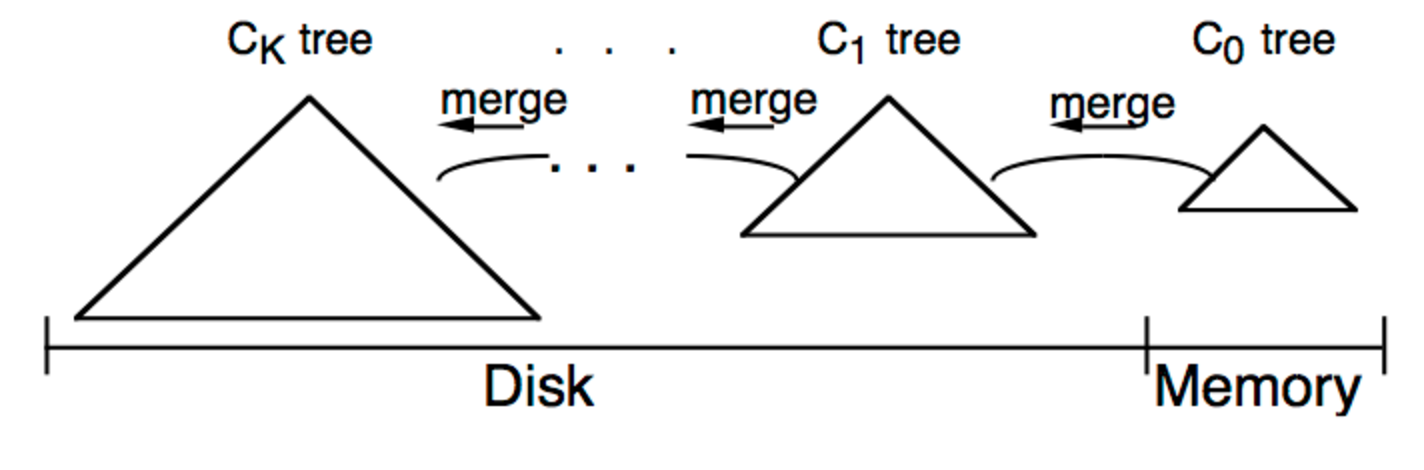
\includegraphics[scale=0.35]{lsm_tree.png}
\caption{LSM Tree structure}
\end{figure}
\end{frame}


\section{Design}

\subsection{Data Structure}

\begin{frame}{Layers Architecture}
\begin{figure}[H]
\begin{center}
    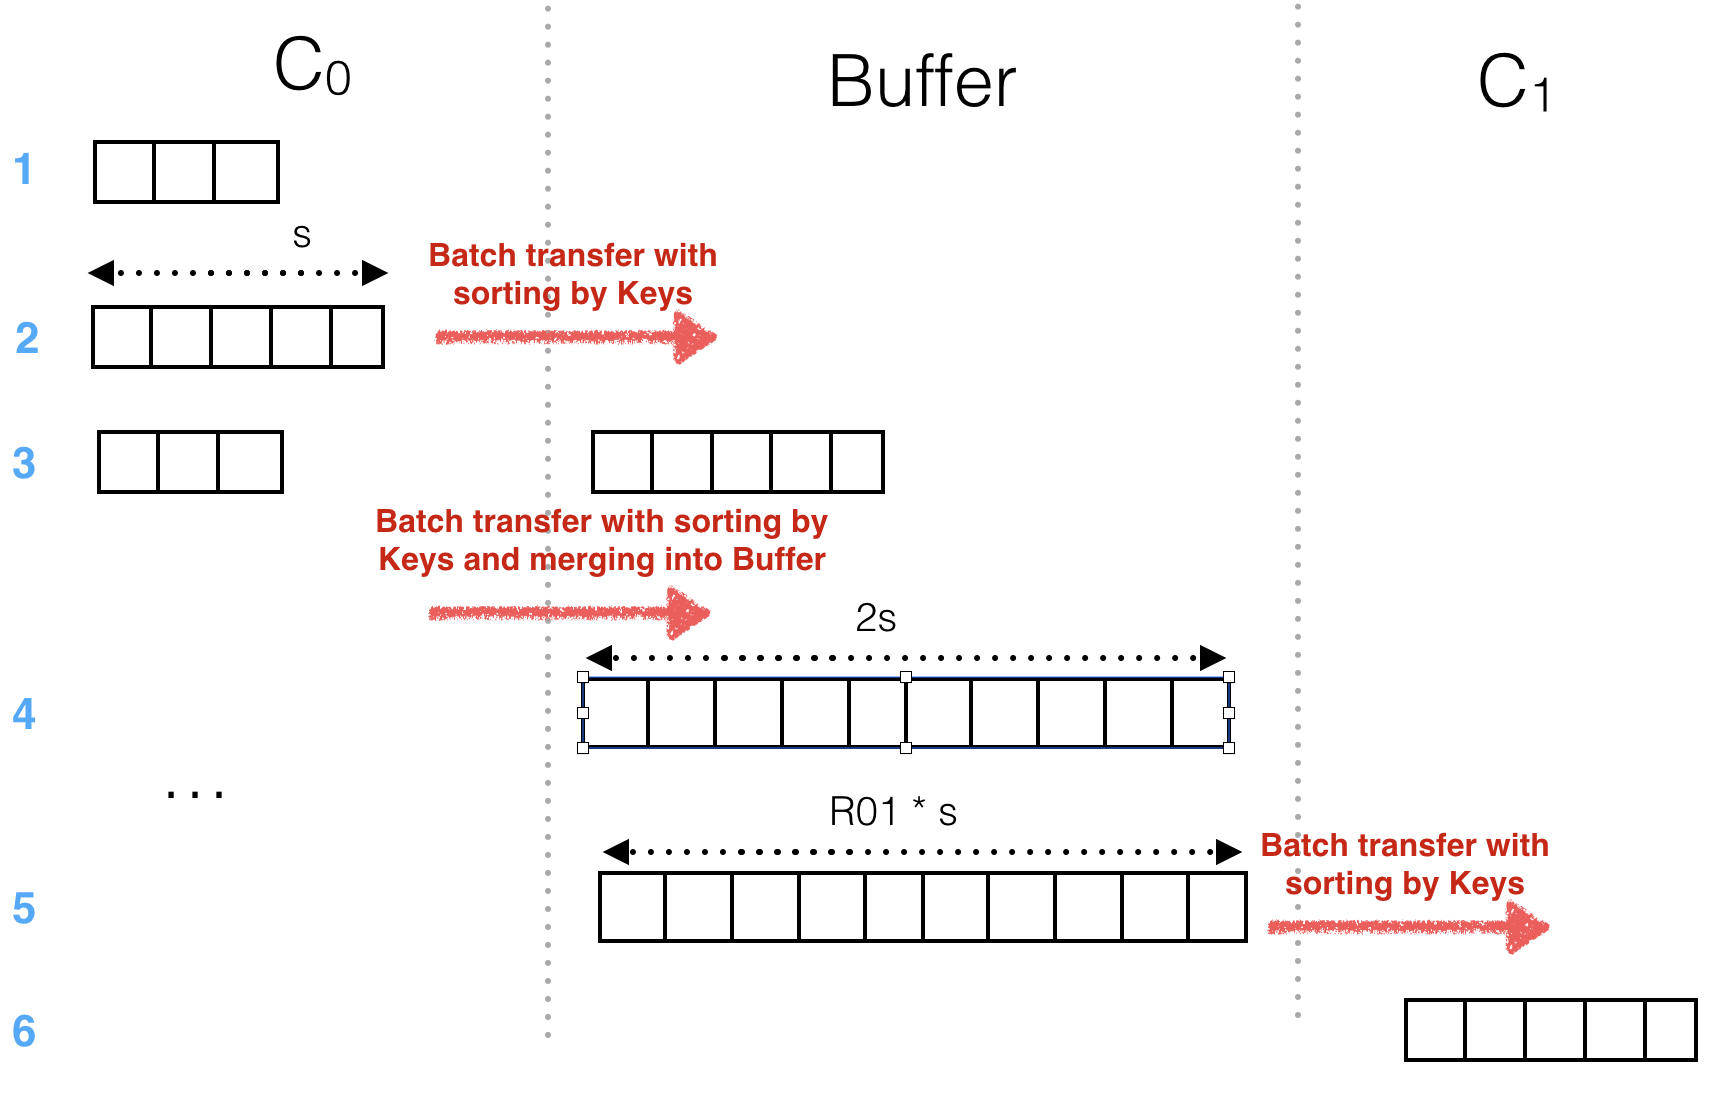
\includegraphics[width=0.5\textwidth]{merge}
    \caption{Merging Strategy}
\end{center}
\end{figure}
\end{frame}


\subsection{Operations}

\begin{frame}{Operations}
	\begin{itemize}
		\item READ
		\begin{enumerate}
			\item Linear search in $C_0$
			\item binary search in other components
		\end{enumerate}				
		\item APPEND (insert, update, delete)
		\begin{enumerate}
			\item Linear search in $C_0$ (removing/updating keys)
			\item Merging if full
		\end{enumerate}	
	\end{itemize}
\end{frame}


\subsection{Persistency}

\begin{frame}
Each component contains two arrays: keys and values.

$C_0$ and buffer on memory
\end{frame}



\subsection{Implementation details}

\begin{frame}{Optimizations}
\begin{itemize}
	\item Memory Mapped File
	\item Bounds Check
	\item Fault tolerance strategy
	\item Bloom Filter
\end{itemize}
\end{frame}

\subsection{Parallel Reads}

\begin{frame}{Parallel Design}
Two approaches are considered:
\begin{itemize}
	\item Killing threads operating on deeper component once the key is found in its lowest component.
	\item Threads communication through a shared variable storing the lowest component on which the key has been found so far
\end{itemize}
\end{frame}



\subsection{Alternative Merging Strategy}

\begin{frame}
\begin{figure}[H]
\begin{center}
    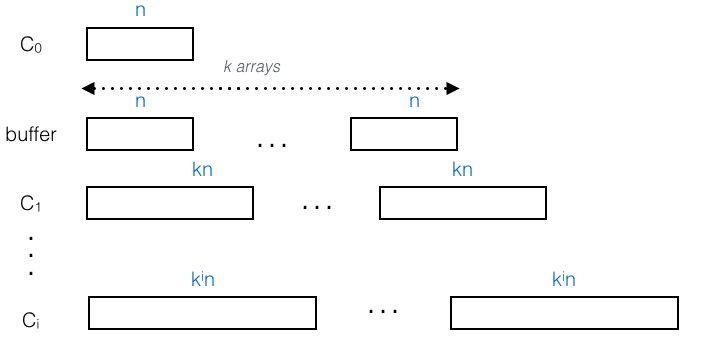
\includegraphics[width=0.4\textwidth]{varlsm}
    \caption{Alternative Merging Strategy}
\end{center}
\end{figure}
\end{frame}

\section{Experiments}

\begin{frame}{Set Up}
\begin{itemize}
	\item 1 000 000 keys inserted
	\item keys are int, values string of size 32
\end{itemize}
\end{frame}

\begin{frame}{Set Up}

5 different LSM structures used:
\begin{enumerate}
	\item $C_0$ size = 1000; size ratios  = 3
	\item $C_0$ size = 2000; size ratios = 3
	\item $C_0$ size = 1000; size ratios = 3 and then 9
	\item $C_0$ size = 1000; size ratios = 5
	\item $C_0$ size = 500; size ratios = 5
\end{enumerate}

\end{frame}

\begin{frame}{Results}
     \begin{columns}[T] % contents are top vertically aligned
     \begin{column}[T]{6cm} % each column can also be its own environment
     \begin{center}
\begin{figure}[H]
\begin{center}
    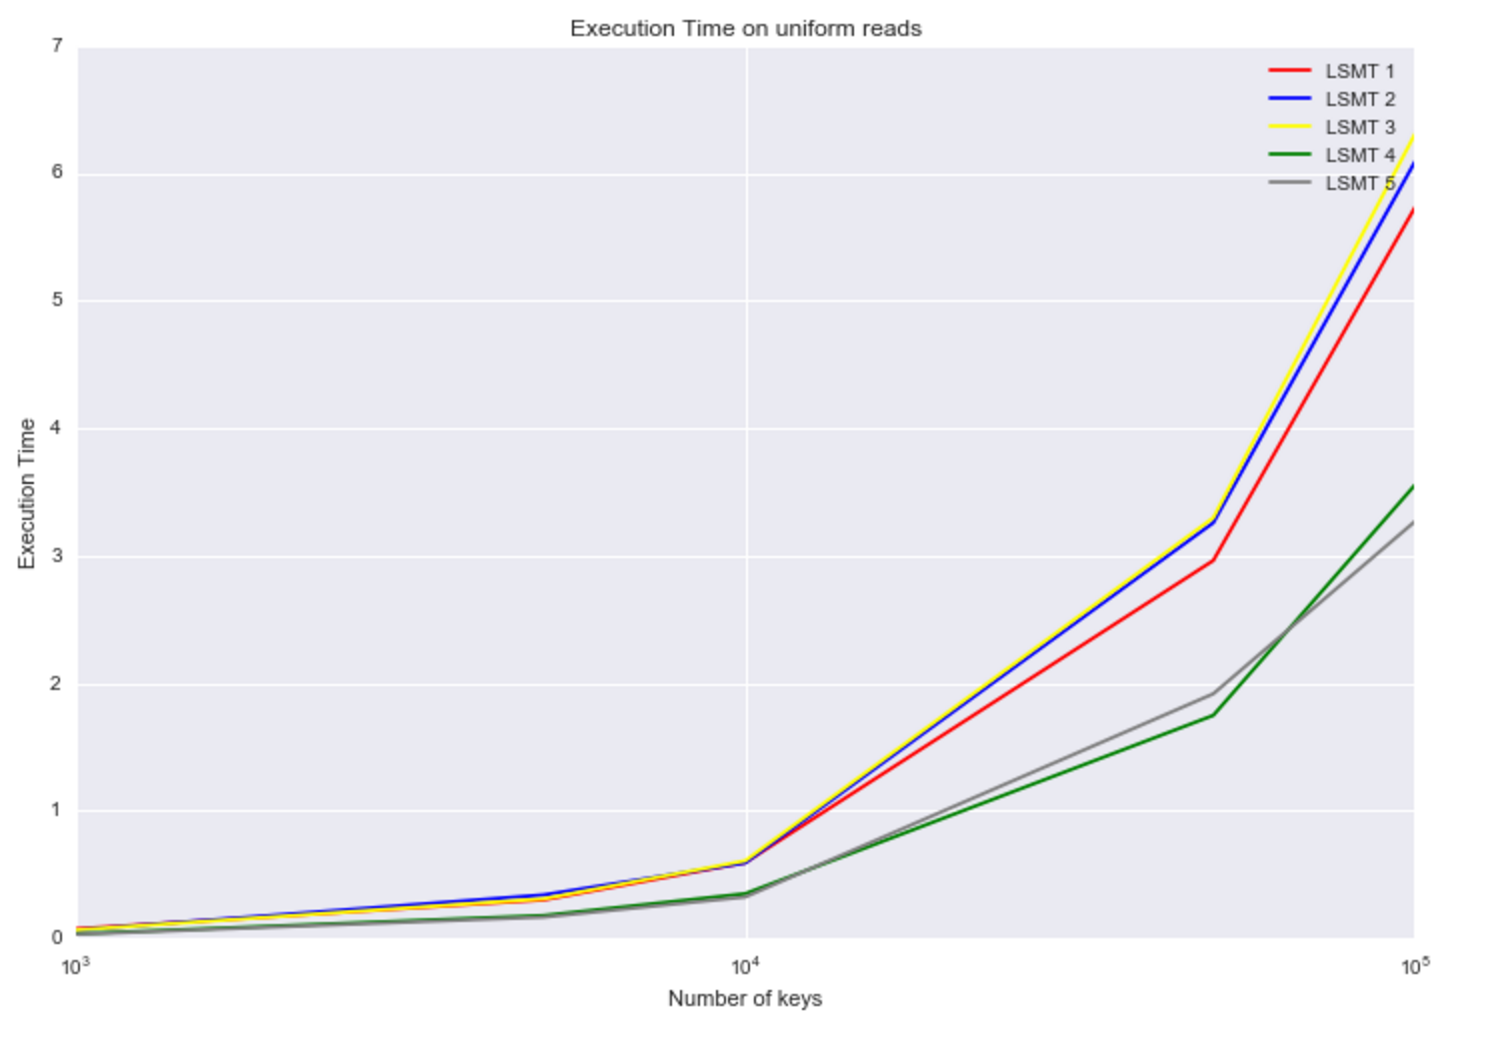
\includegraphics[width=0.7\textwidth]{reads_unif}
    \caption{Uniform Reads}
\end{center}
\end{figure}
	\end{center}
     \end{column}
          \begin{column}[T]{6cm} % alternative top-align that's better for graphics
\begin{figure}[H]
\begin{center}
    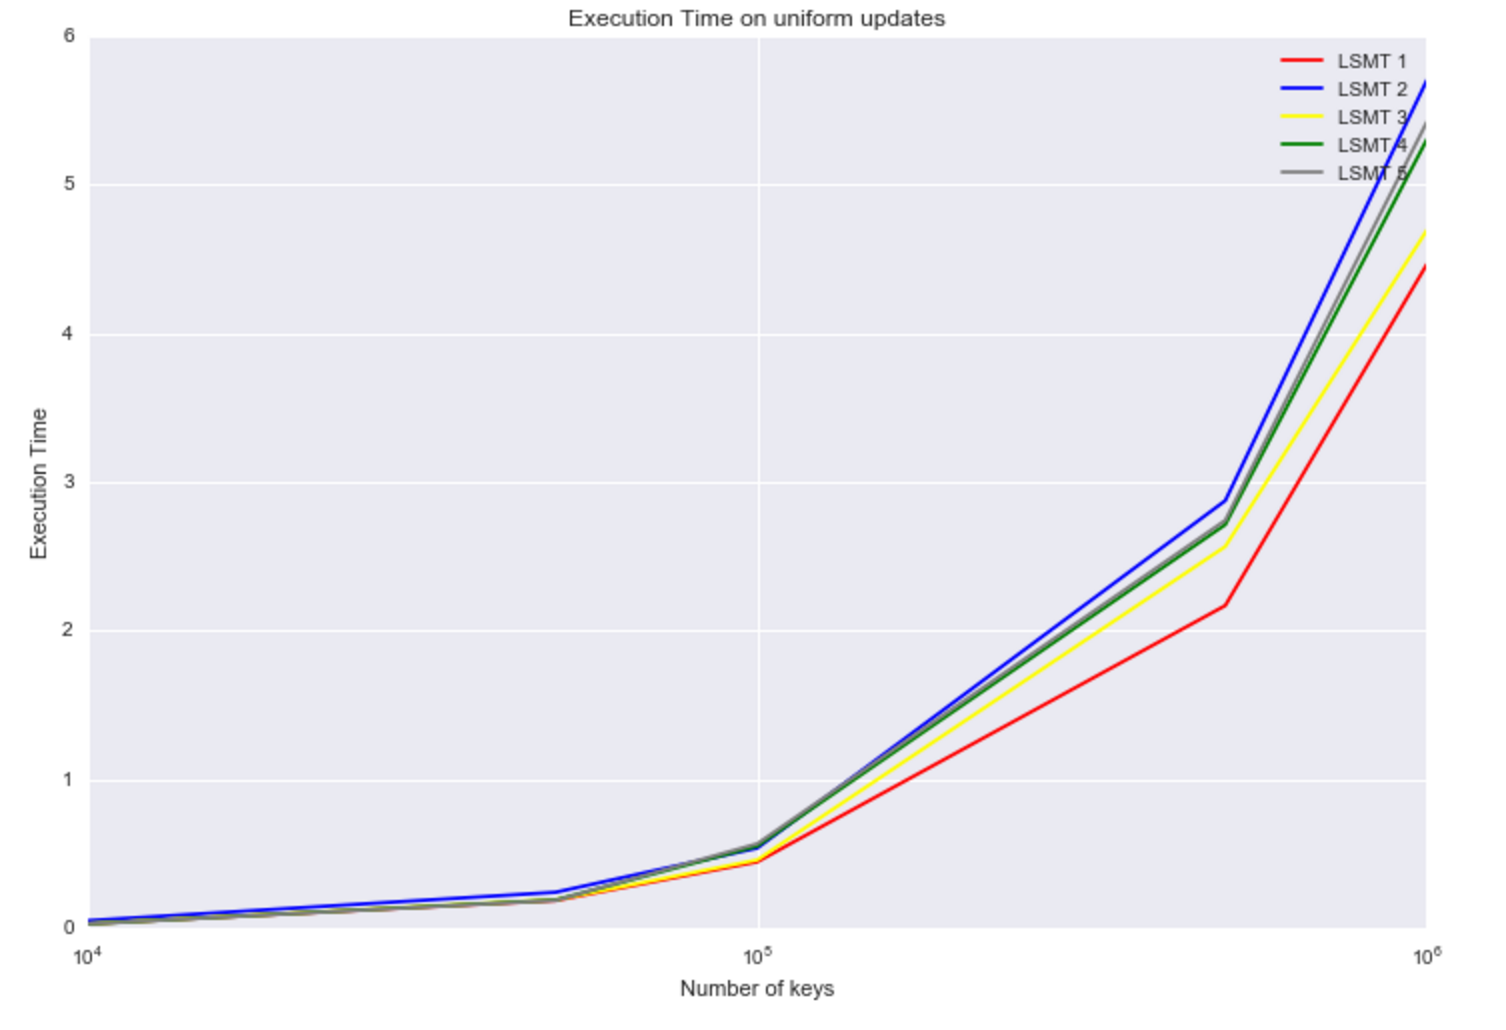
\includegraphics[width=0.7\textwidth]{updates_unif}
    \caption{Uniform Updates}
\end{center}
\end{figure}
    	\end{column}
     \end{columns}
\end{frame}

\begin{frame}{Results}
     \begin{columns}[T] % contents are top vertically aligned
     \begin{column}[T]{6cm} % each column can also be its own environment
     \begin{center}
\begin{figure}[H]
\begin{center}
    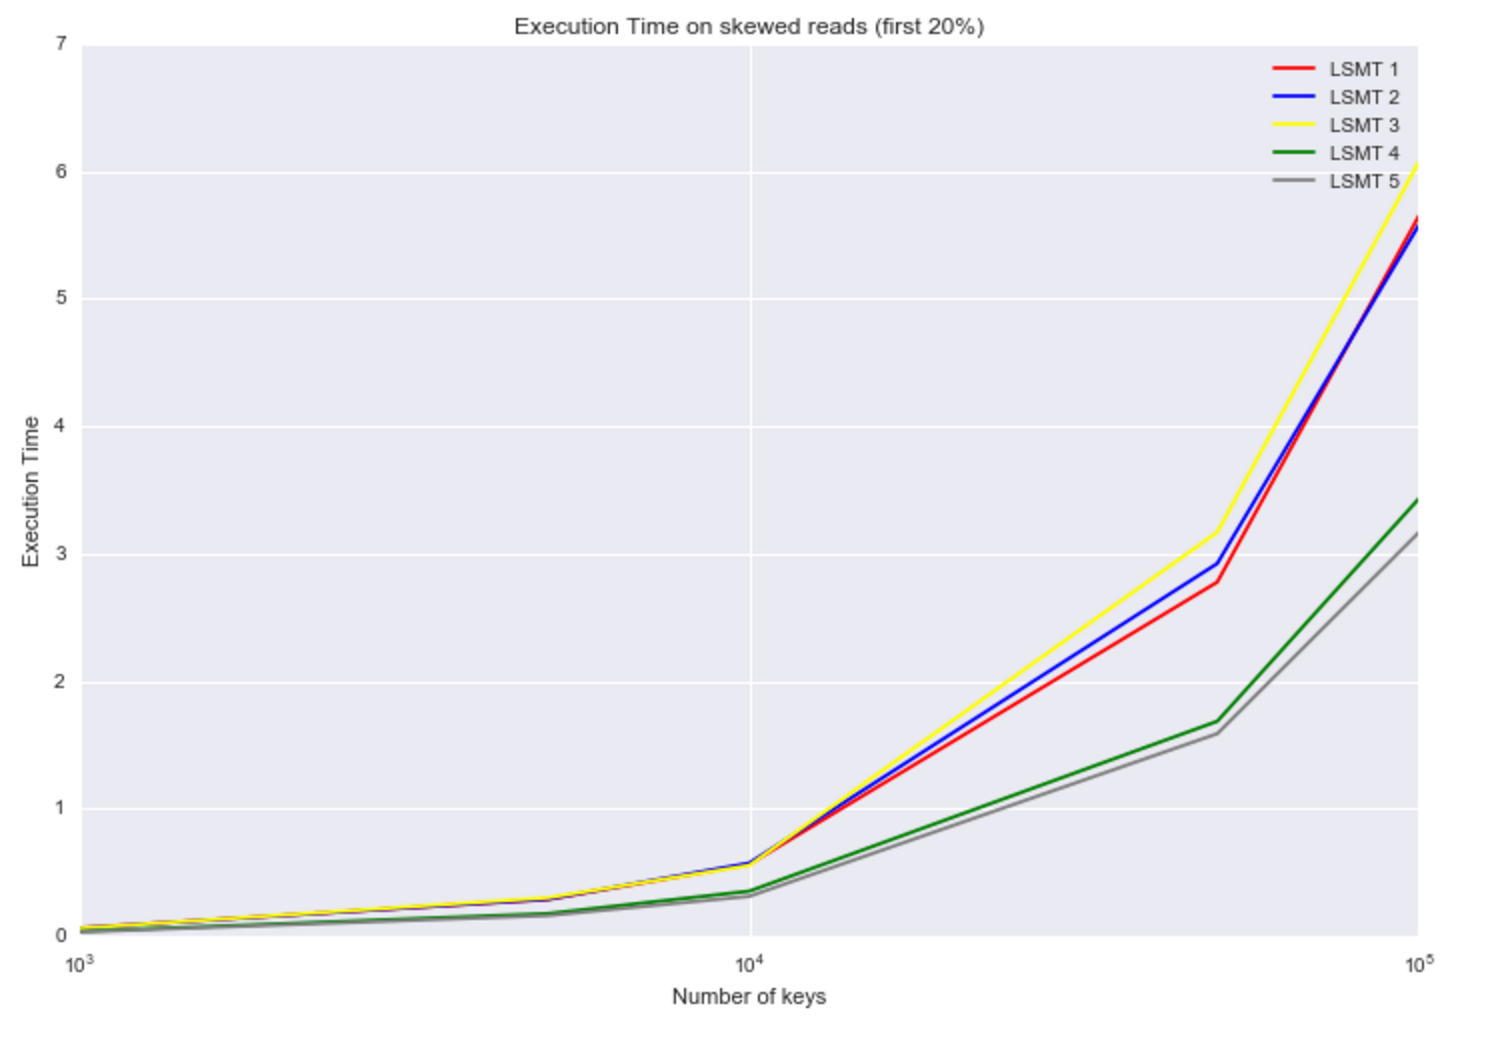
\includegraphics[width=0.7\textwidth]{reads_skbeg}
    \caption{Skewed reads (20\% start)}
\end{center}
\end{figure}
	\end{center}
     \end{column}
          \begin{column}[T]{6cm} % alternative top-align that's better for graphics
\begin{figure}[H]
\begin{center}
    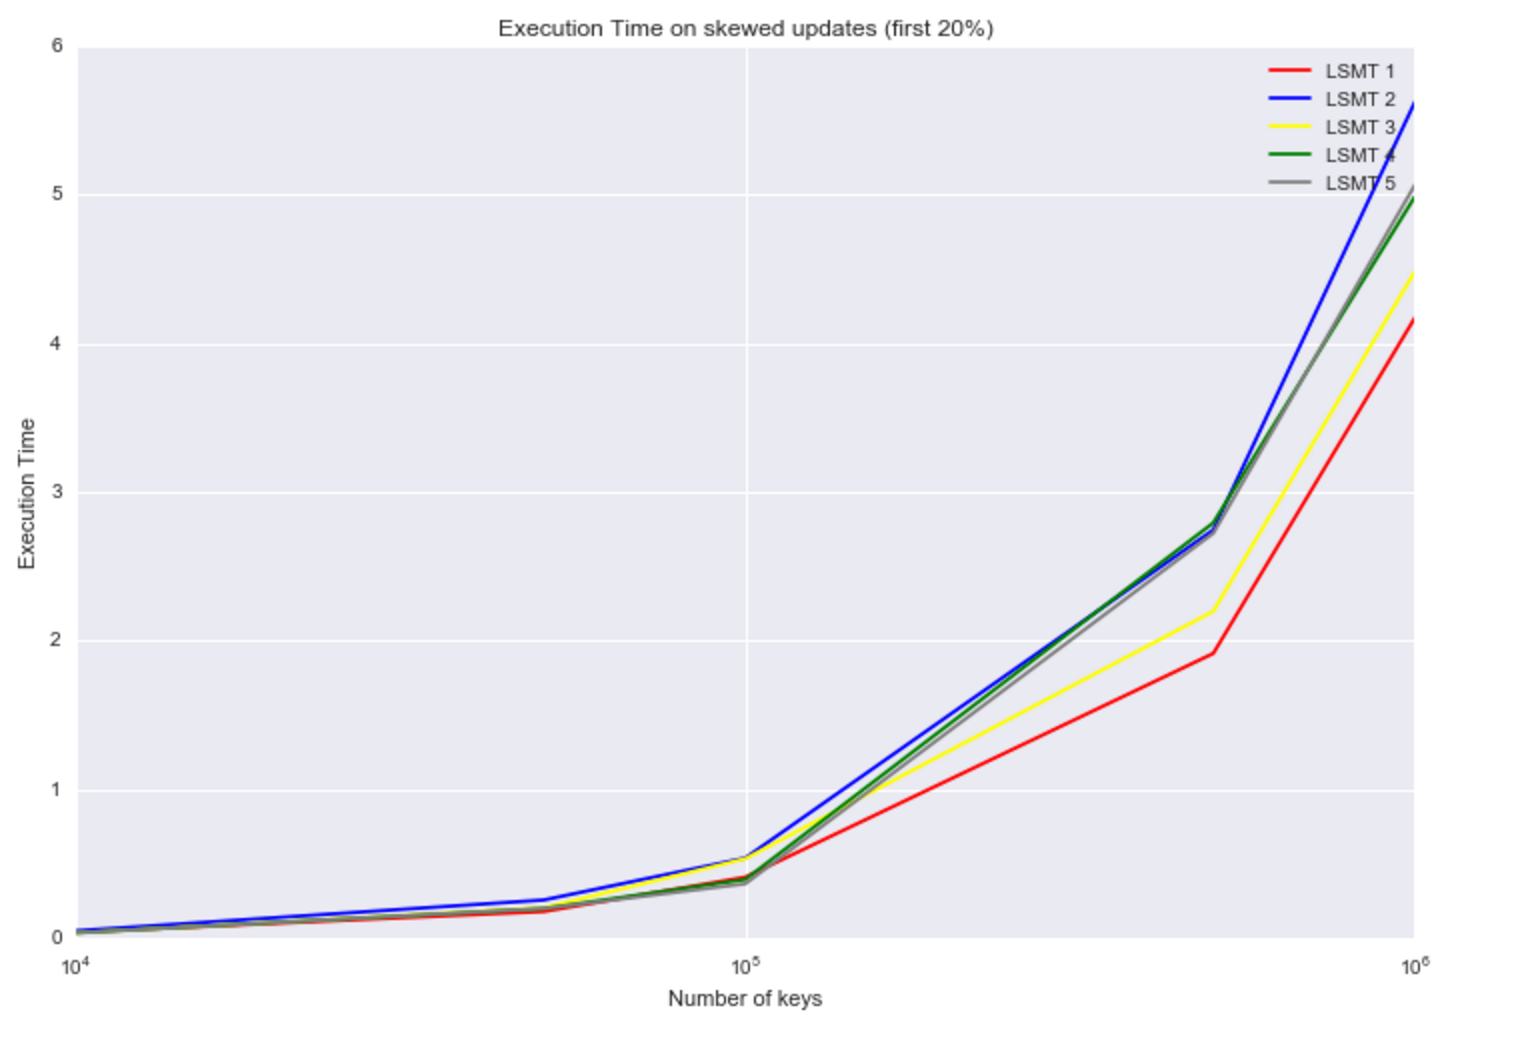
\includegraphics[width=0.7\textwidth]{updates_skbeg}
    \caption{Skewed updates (20\% start)}
\end{center}
\end{figure}
    	\end{column}
     \end{columns}
\end{frame}

\begin{frame}{Results}
     \begin{columns}[T] % contents are top vertically aligned
     \begin{column}[T]{6cm} % each column can also be its own environment
     \begin{center}
\begin{figure}[H]
\begin{center}
    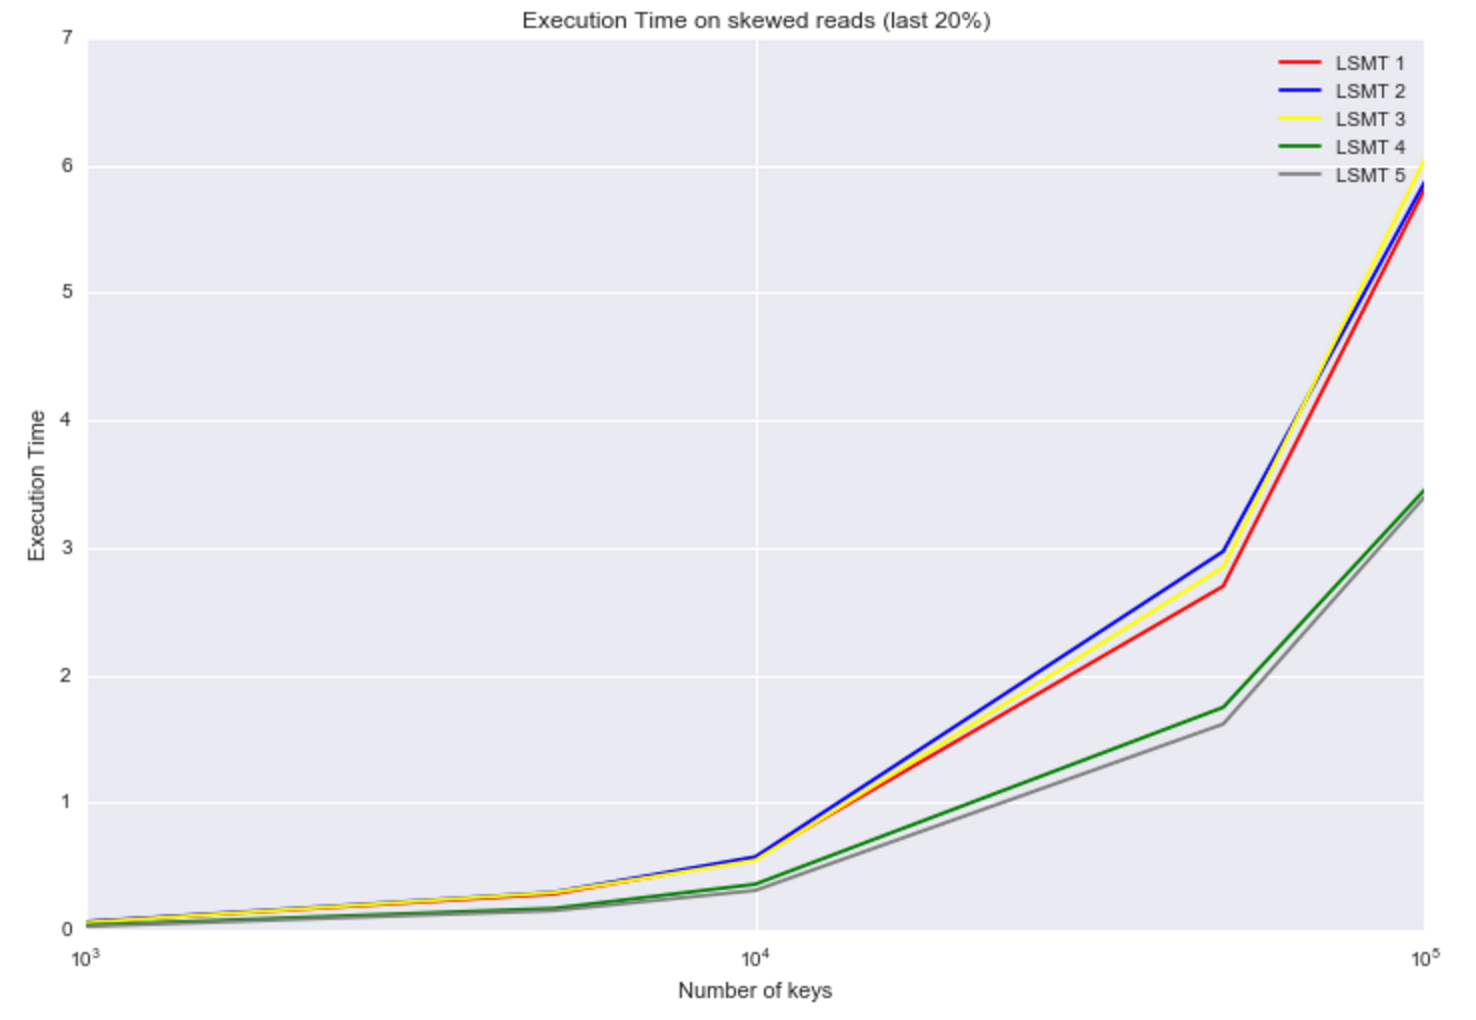
\includegraphics[width=0.7\textwidth]{reads_skend}
    \caption{Skewed reads (20\% end)}
\end{center}
\end{figure}
	\end{center}
     \end{column}
          \begin{column}[T]{6cm} % alternative top-align that's better for graphics
\begin{figure}[H]
\begin{center}
    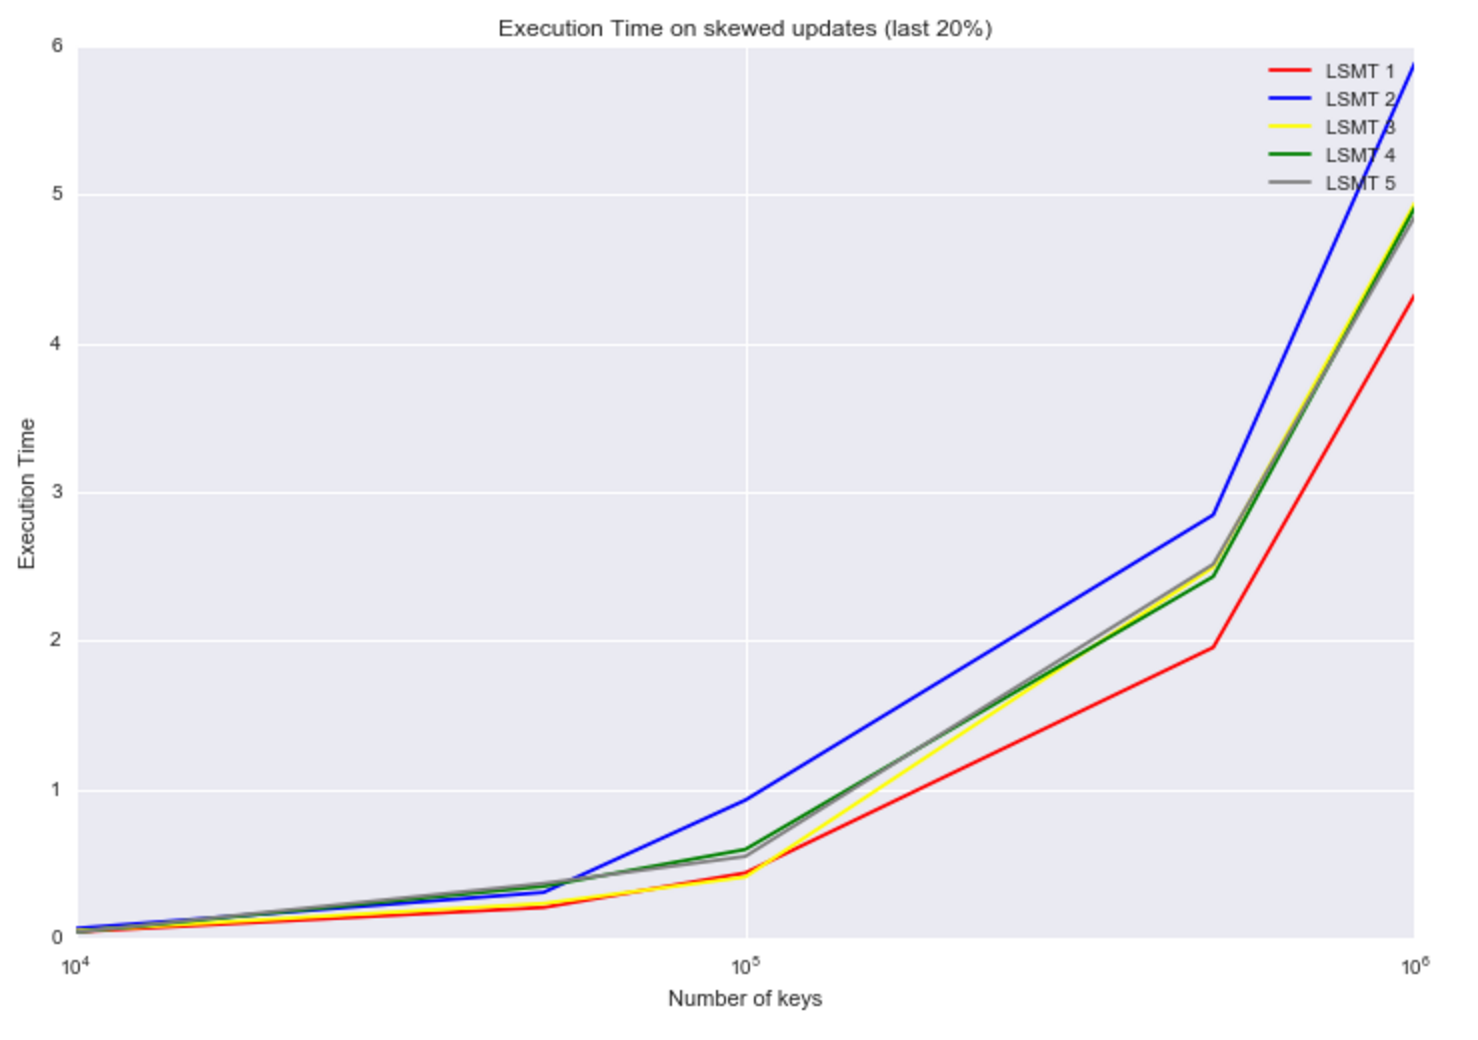
\includegraphics[width=0.7\textwidth]{updates_skend}
    \caption{Skewed updates (20\% end)}
\end{center}
\end{figure}
    	\end{column}
     \end{columns}
\end{frame}

\begin{frame}{Results}
\begin{figure}[H]
\begin{center}
    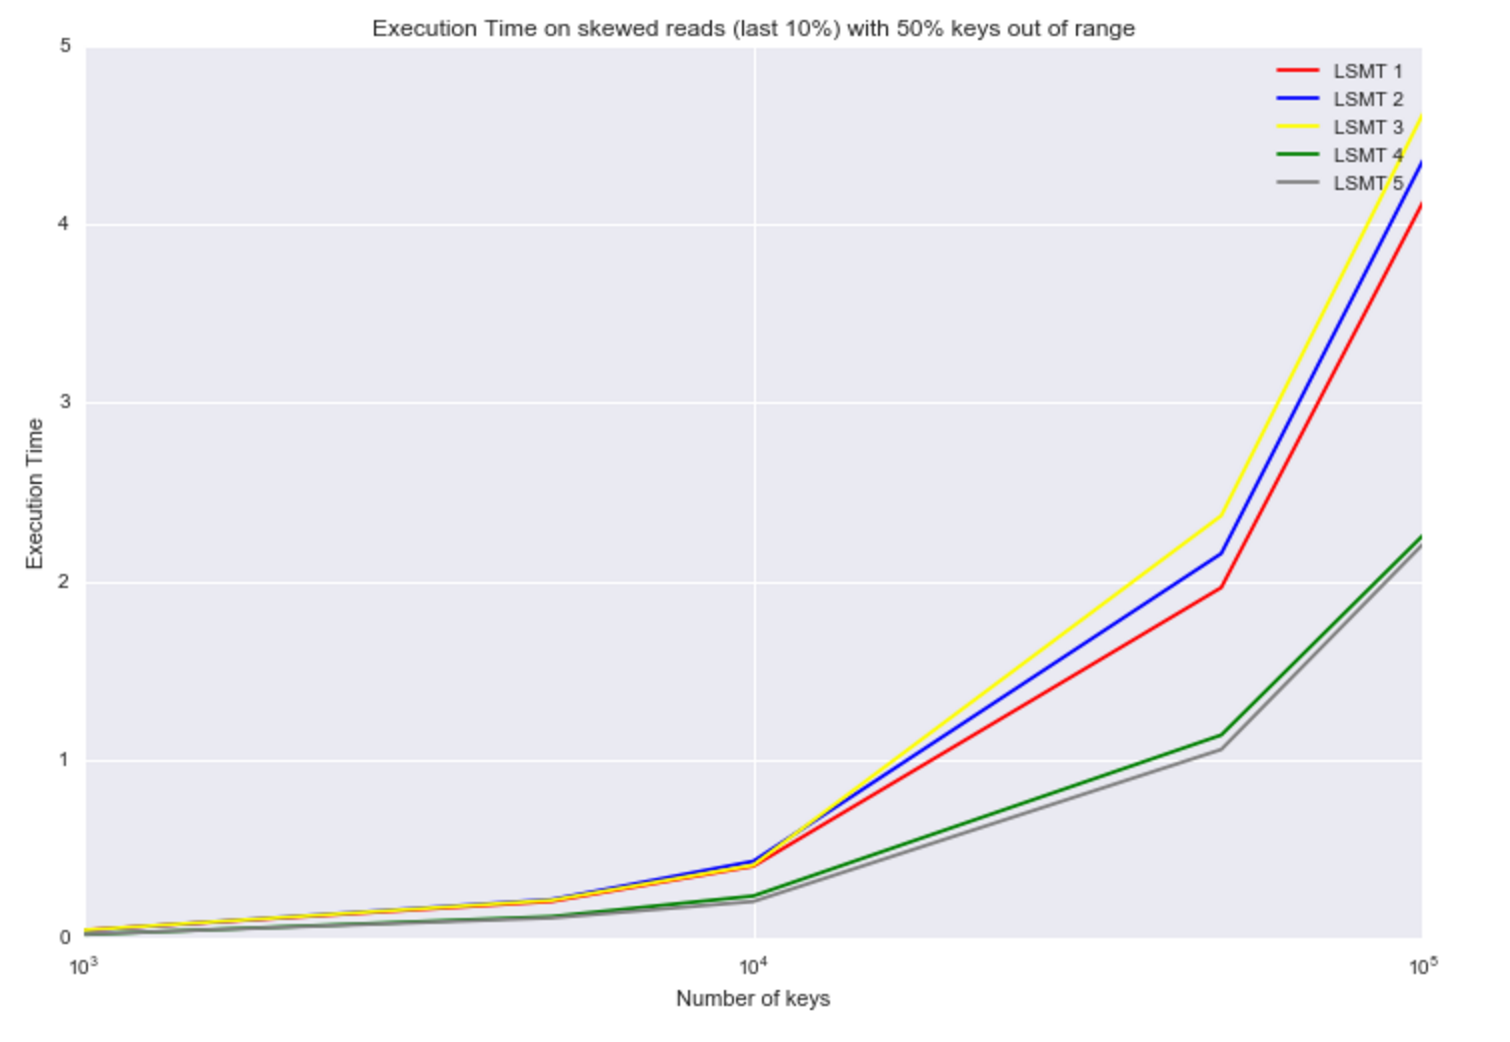
\includegraphics[width=0.7\textwidth]{reads_skout}
    \caption{Skewed reads (10\% end) and 50\% out of range}
\end{center}
\end{figure}

\end{frame}


\section{Future Steps}

\begin{frame}
\begin{itemize}
	\item Experiments on Bloom Filter and Parallel implementation
	\item Possibility to choose the merging strategy
\end{itemize}
\end{frame}




\end{document}